\section{Competitors Analysis}\label{sect:CompetitorsAnalysis}In this chapter, we present the Competitor Analysis, which is a fundamental step in the design process of TrainHub. Before developing our application, we researched the current market to understand how other companies have tackled similar problems and to identify areas where our project could stand out.

To conduct this analysis, we searched the main mobile stores (Google Play Store and Apple App Store) for apps related to fitness and gym management. We selected a few key applications, downloaded them, and tested their main functionalities.

For comparison purposes, we divided the analyzed applications into two main categories:
\begin{itemize}
    \item \textbf{Direct Competitors: }applications that try to solve the same problem, with the same value proposition, for the same target users;
    \item \textbf{Indirect Competitors: }applications that target a similar user group but with a different value proposition, or vice versa.
\end{itemize}

Overall, this study allowed us to identify the strengths and weaknesses of the current solutions on the market. By understanding what is already available, we were able to define the core features of TrainHub and highlight how our app can solve problems that others currently ignore.
\subsection{Direct Competitors}\label{subsect:DirectCompetitors}
For TrainHub, direct competitors are applications that are strictly tied to a physical gym environment. These apps aim to provide an all-in-one ecosystem that connects gym members with the facility and its professionals. Their main goal is to centralize the user's gym experience, offering tools such as digital access, course bookings, and training programs within a single platform.

Based on our market research, we identified four key players in this category. These include applications developed specifically for major gym chains, generalized management software widely used by local gyms, and global industry benchmarks that offer comprehensive business-to-business (B2B) and business-to-consumer (B2C) solutions.

To properly evaluate these competitors, we summarized our findings in the following two comparison tables:
\begin{itemize}
    \item \textbf{Dimensions Table:} this table compares general market aspects, such as the business model, pricing, and user ratings on digital stores, helping us understand the scale of these competitors;
    \item \textbf{Features Table:} this table breaks down the specific functionalities offered by each application.
\end{itemize}

By mapping out what these apps currently offer, we can clearly highlight the gaps in the market, such as the lack of fully integrated diet management and direct chat with professionals, and demonstrate how TrainHub can provide a more complete and seamless experience for both clients and gym staff.

\paragraph{Virgin Active}The Virgin Active app is the official mobile application for members of the Virgin Active gym chain. It provides an exclusive ecosystem that allows users to easily book classes, access remote training sessions, and stay updated on club news. Additionally, it offers practical tools to follow daily workouts, monitor personal performance, and track fitness progress in a centralized and interactive way.

\begin{figure}[H]
    \centering
    \begin{subfigure}{0.4\textwidth}
        \centering
        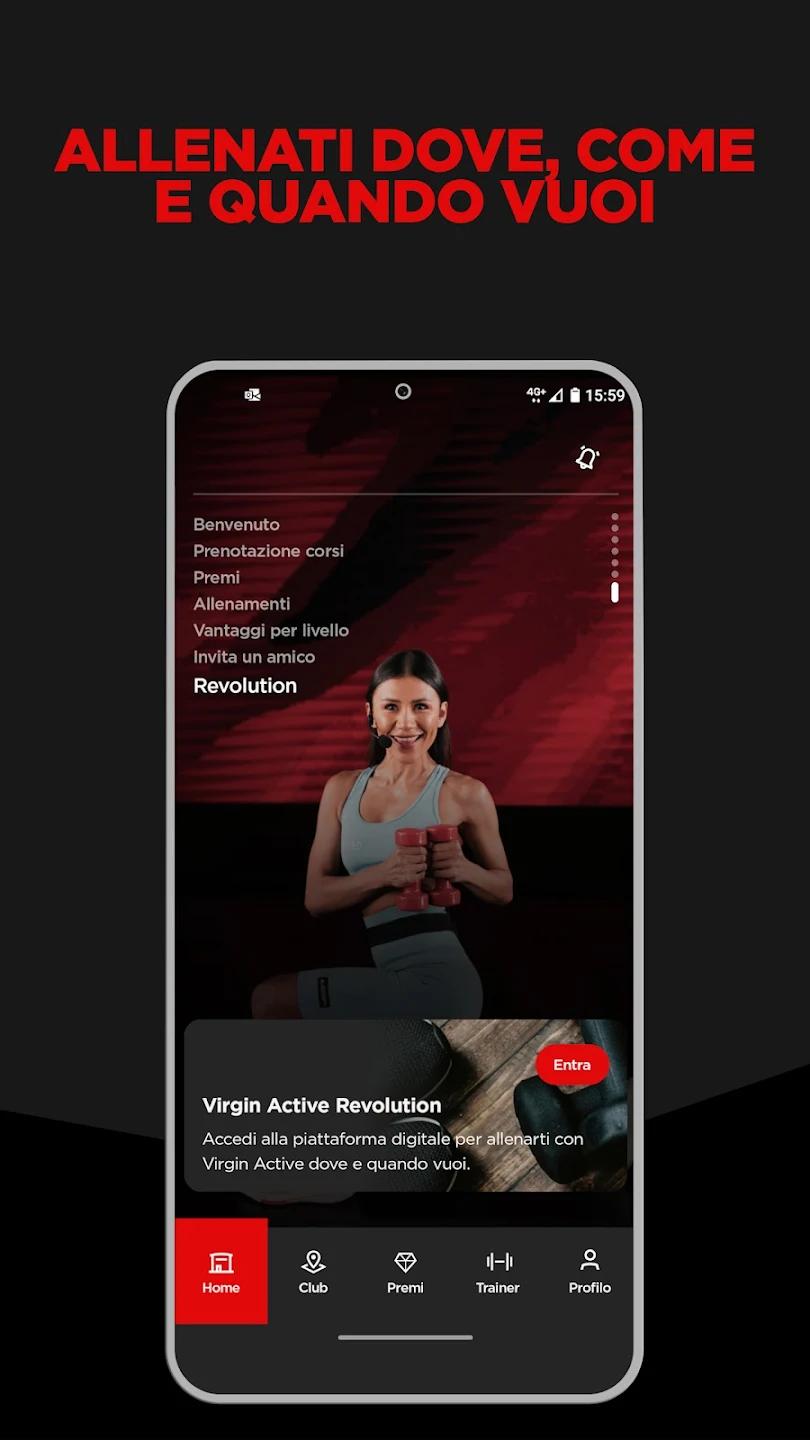
\includegraphics[width=\textwidth]{2-CompetitorsAnalysis/img/VirginActive/Home.jpg}
        \caption{Home Interface}
        \label{fig:virgin_home}
    \end{subfigure}
    % \hfill
    \begin{subfigure}{0.4\textwidth}
        \centering
        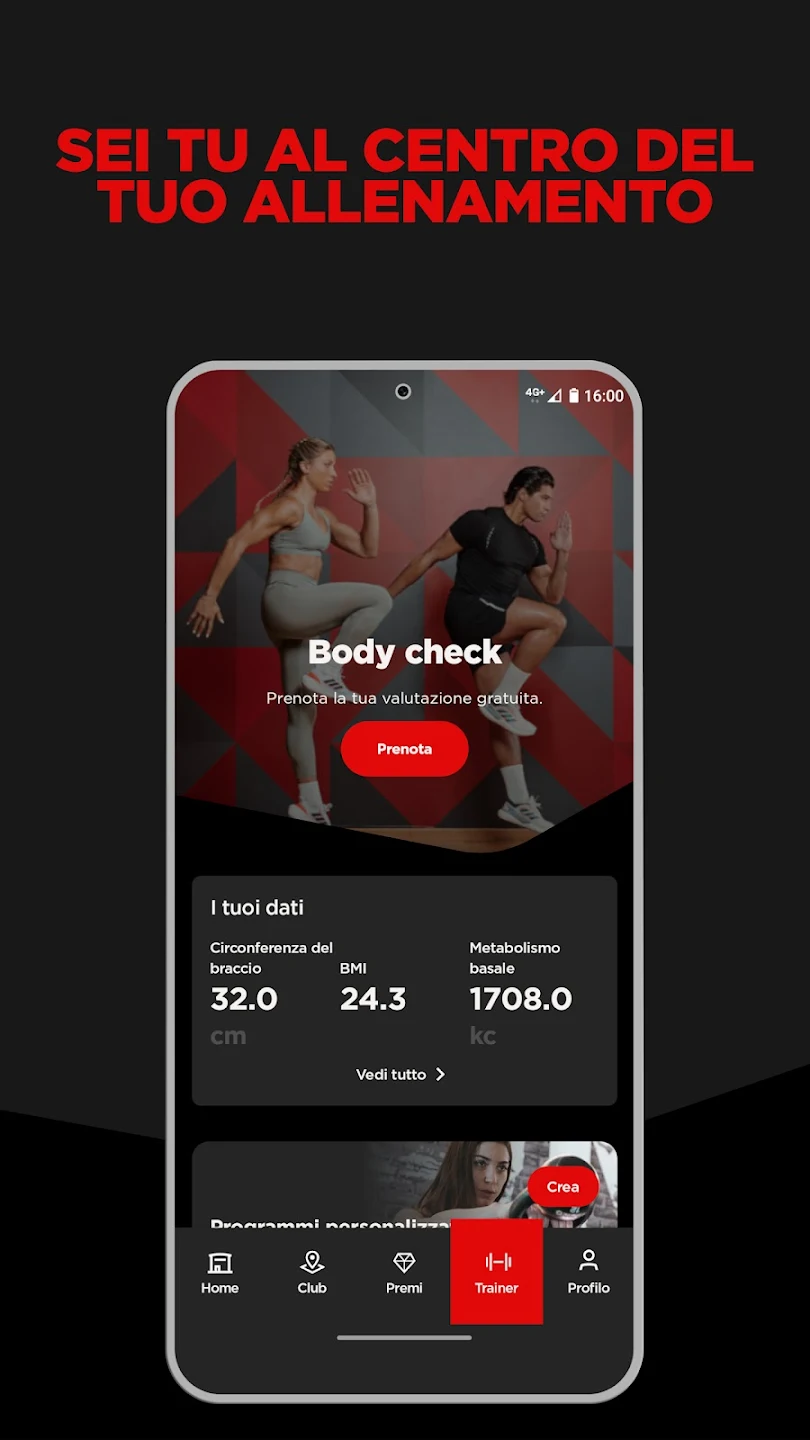
\includegraphics[width=\textwidth]{2-CompetitorsAnalysis/img/VirginActive/Trainer.jpg}
        \caption{Trainer Interface}
        \label{fig:virgin_trainer}
    \end{subfigure}
    \caption{Virgin Active App Interface}
    \label{fig:virgin_active_app}
\end{figure}

\paragraph{EvolutionFit Club}EvolutionFit is a comprehensive management application designed for both gym clients and personal trainers. It provides an all-in-one solution that integrates workout plan management, facility and class bookings, and detailed progress tracking. Furthermore, it features a dedicated nutrition section with a food diary and calorie goals, aiming to centralize the user's entire fitness and dietary journey into a single platform.

\begin{figure}[H]
    \centering
    \begin{subfigure}{0.4\textwidth}
        \centering
        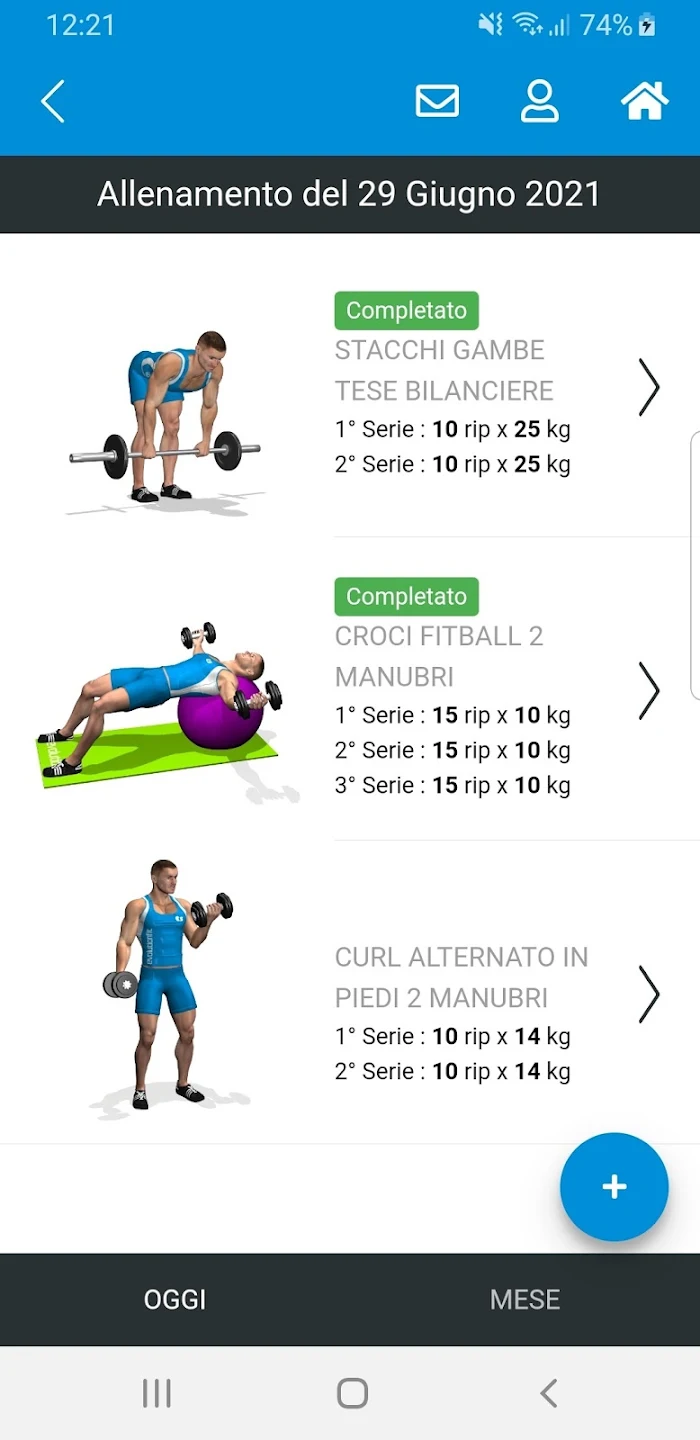
\includegraphics[width=\textwidth]{2-CompetitorsAnalysis/img/EvolutionFit/Workout.jpg}
        \caption{Workout Interface}
        \label{fig:evolution_workout}
    \end{subfigure}
    % \hfill
    \begin{subfigure}{0.4\textwidth}
        \centering
        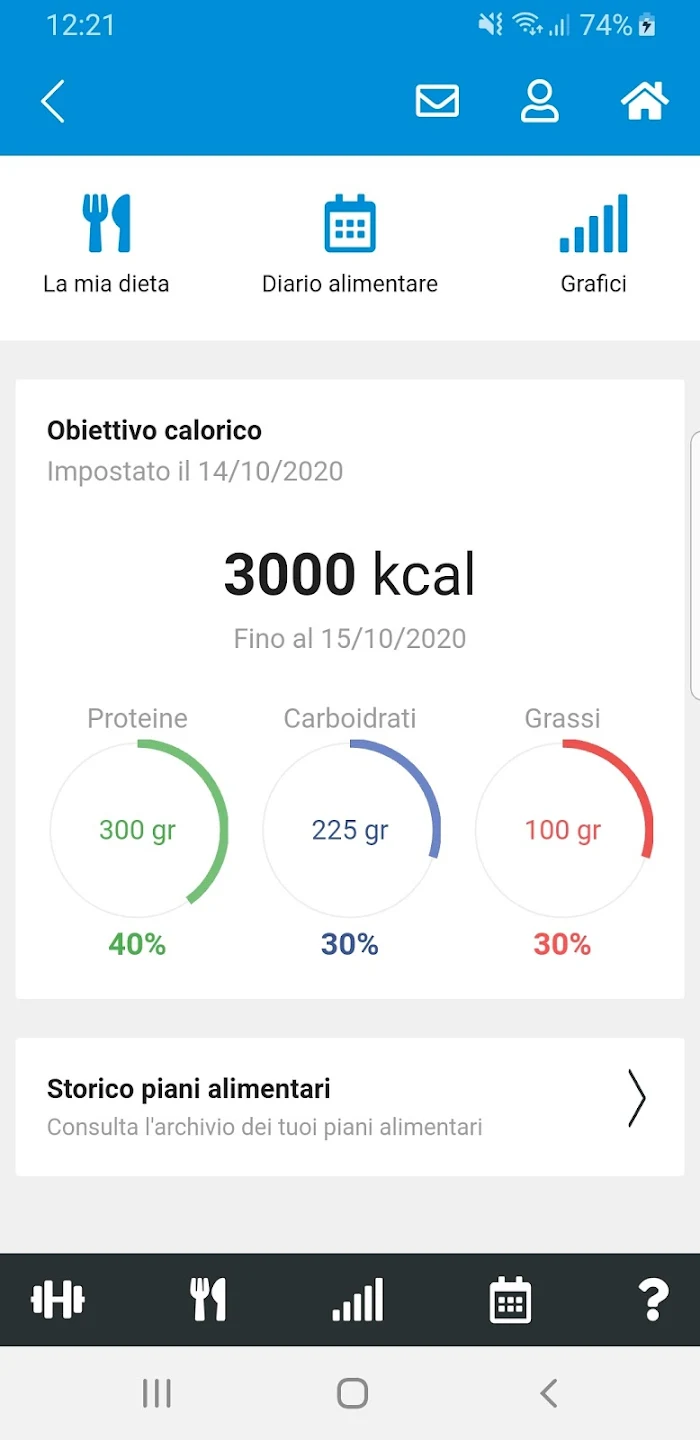
\includegraphics[width=\textwidth]{2-CompetitorsAnalysis/img/EvolutionFit/Nutrition.jpg}
        \caption{Nutrition Interface}
        \label{fig:evolution_nutrition}
    \end{subfigure}
    \caption{EvolutionFit App Interface}
    \label{fig:evolution_fit_app}
\end{figure}

\paragraph{Technogym}The Technogym App is a robust health and fitness platform powered by an AI Coach that generates customized training programs based on user goals, available time, and equipment. It features a vast library of over 1,000 on-demand workouts, holistic wellness content, and community challenges. The app also strongly focuses on performance monitoring by seamlessly syncing with major third-party wearables and health trackers.

\begin{figure}[H]
    \centering
    \begin{subfigure}{0.4\textwidth}
        \centering
        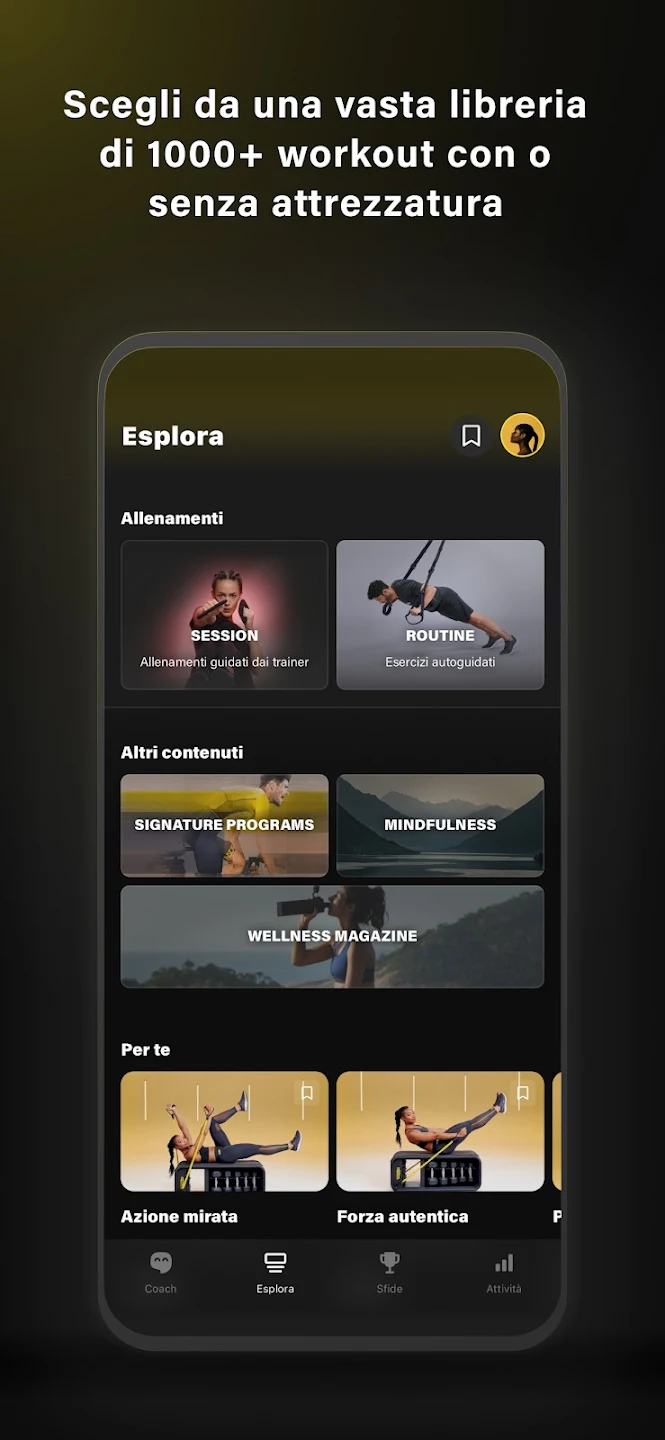
\includegraphics[width=\textwidth]{2-CompetitorsAnalysis/img/Technogym/Explore.jpg}
        \caption{Workout Interface}
        \label{fig:technogym_explore}
    \end{subfigure}
    % \hfill
    \begin{subfigure}{0.4\textwidth}
        \centering
        
\includegraphics[width=\textwidth]{2-CompetitorsAnalysis/img/Technogym/Challenge.jpg}
        \caption{Challenge Interface}
        \label{fig:technogym_challenge}
    \end{subfigure}
    \caption{Technogym App Interface}
    \label{fig:technogym_app}
\end{figure}


\paragraph{Virtualgym}Virtuagym is a highly versatile fitness platform featuring an extensive database of over 4,000 exercises suitable for various fitness levels, locations, and equipment availability. A standout feature is its deep integration with its sister application, Virtuagym Food, which provides advanced macronutrient and calorie tracking. Together, they offer a complete ecosystem for both workout management and nutritional planning, supported by wearable integrations.

\begin{figure}[H]
    \centering
    \begin{subfigure}{0.4\textwidth}
        \centering
        
\includegraphics[width=\textwidth]{2-CompetitorsAnalysis/img/Virtualgym/Workout.jpg}
        \caption{Workout Interface}
        \label{fig:virtualgym_workout}
    \end{subfigure}
    % \hfill
    \begin{subfigure}{0.4\textwidth}
        \centering
        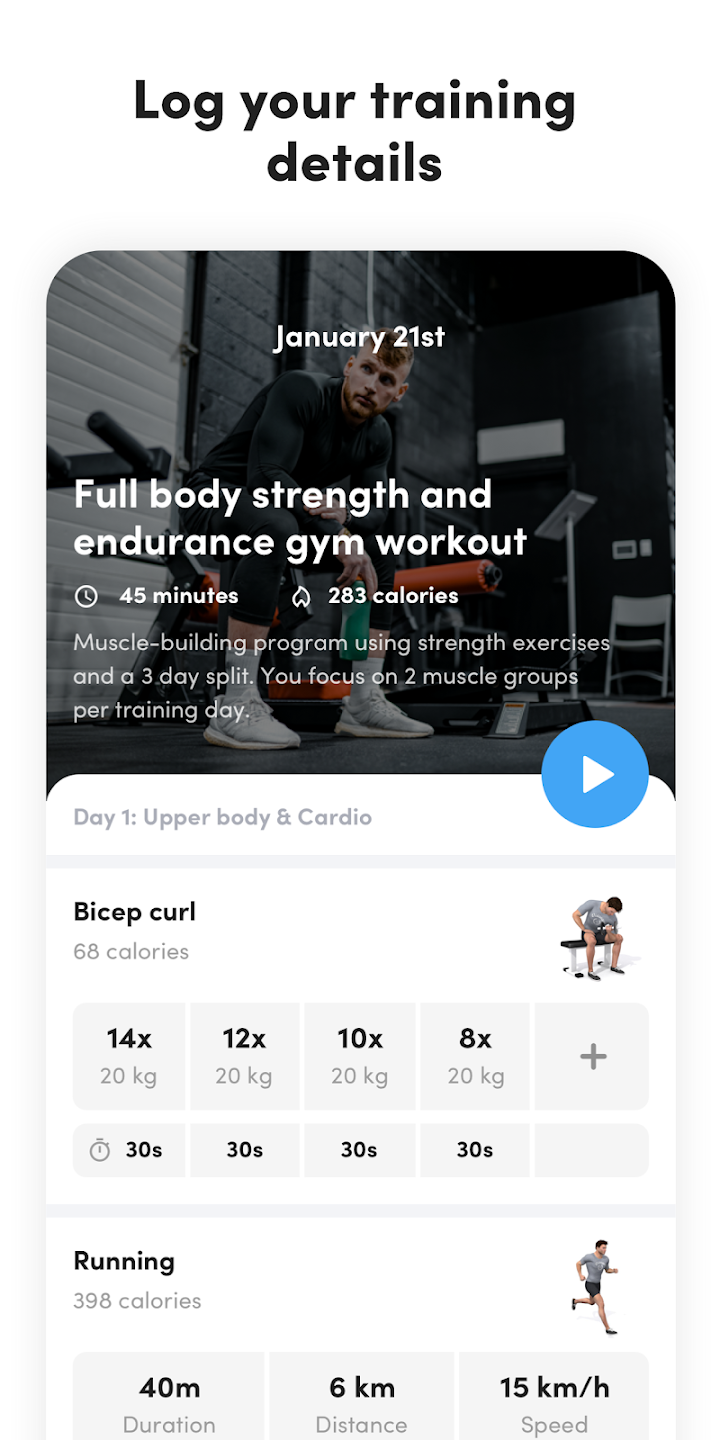
\includegraphics[width=\textwidth]{2-CompetitorsAnalysis/img/Virtualgym/Log.jpg}
        \caption{Log Interface}
        \label{fig:virtualgym_log}
    \end{subfigure}
    \caption{Virtualgym App Interface}
    \label{fig:virtualgym_app}
\end{figure}

\begin{table}[H]
    \centering
    \resizebox{\textwidth}{!}{
    \begin{tabular}{l c c c c}
        \toprule
        \textbf{Dimension} & \textbf{Virgin Active} & \textbf{EvolutionFit} & \textbf{Technogym} & \textbf{Virtuagym} \\
        \midrule
        Business Model / Price       & Included in Membership & Free for Users (B2B) & Freemium / Subs & Freemium / Subs \\
        Registration                 & Mandatory & Mandatory & Mandatory & Mandatory \\
        Target Audience              & Virgin Active Members & Affiliated Gym Members & B2B / B2C (All) & B2B / B2C (All) \\
        Supported Platforms          & iOS, Android & iOS, Android, Web & iOS, Android, Watch & iOS, Android, Web \\
        Downloads (Play Store)       & 5Mln+ & Not comparable (gym-distributed) & 1Mln+ & 5Mln+ \\
        Rating (Play Store)          & 4.6 & 3.4 & 4.8 & 4.7 \\
        Rating (App Store)           & 4.7 & 2.5 & 4.7 & 4.7 \\
        \bottomrule
    \end{tabular}
    }
    \vspace{0.2cm}
    \caption{Dimensions comparison of direct competitors}
    \label{tab:dimensions_competitors}
\end{table}

\vspace{0.5cm}

\begin{table}[H]
    \centering
    \resizebox{\textwidth}{!}{
    \begin{tabular}{l c c c c}
        \toprule
        \textbf{Feature} & \textbf{Virgin Active} & \textbf{EvolutionFit} & \textbf{Technogym} & \textbf{Virtuagym} \\
        \midrule
        Workout tracking \& statistics       & Yes & Yes & Yes & Yes \\
        Diet \& nutrition management         & No  & Yes & No  & Yes \\
        Class \& appointment booking         & Yes & Yes & Yes & Yes \\
        Digital facility access (QR/RFID)    & Yes & Yes & Yes & Yes \\
        Direct chat with professionals       & No  & Yes & No  & Yes \\
        Dedicated Admin/Staff dashboard      & No  & Yes & Yes & Yes \\
        \bottomrule
    \end{tabular}
    }
    \vspace{0.2cm}
    \caption{Features comparison of direct competitors}
    \label{tab:features_competitors}
\end{table}



\subsection{Indirect Competitors}\label{subsect:IndirectCompetitors}
As defined in our theoretical framework, indirect competitors are applications that target a similar user group but offer a different value proposition, or satisfy only a partial need. For TrainHub, these are applications and tools that focus exclusively on a single aspect of the user's fitness journey (e.g., only diet or only workout tracking) and lack any integration with the services of a physical gym facility.

Our research highlighted a strong fragmentation in the digital habits of gym-goers. We categorized these indirect competitors into four main groups:

\begin{itemize}
    \item \textbf{Workout Tracking (Hevy, GymLife, Bodymatica):}
    these applications allow users to build custom workout routines and track their weightlifting progress.
    \textit{Why they are indirect:} they operate as excellent standalone diaries, but they do not offer a direct, integrated communication channel with the user's actual Personal Trainer, nor do they support facility-specific features like class bookings or gym access;

    \item \textbf{Nutrition Tracking (MyFitnessPal, Yazio):}
    these are market leaders in their specific niche, highly specialized in calorie counting and macronutrient tracking.
    \textit{Why they are indirect:} they focus exclusively on the dietary aspect of fitness, completely detached from the user's workout routines and the gym's ecosystem;

    \item \textbf{Cardio \& General Tracking (Garmin Connect, Strava, Polar Flow, Suunto):}
    these platforms are deeply tied to wearable devices (smartwatches) and excel at tracking outdoor activities, heart rate, and overall health metrics.
    \textit{Why they are indirect:} they are generic health trackers. While extremely useful, they are entirely disconnected from the specific concepts of "gym management", "PT appointments", or "facility interaction";

    \item \textbf{Generic \& Analog Tools (Apple Notes, Excel/Numbers, PDFs, WhatsApp/Telegram, Emails):}
    interestingly, our market research revealed that a significant portion of both clients and professionals still rely heavily on these non-specific tools to log progress, share workout PDFs, and communicate. 
    \textit{Why they are indirect:} they represent the current, inefficient "status quo." Using three or four different generic apps to manage one fitness journey creates friction.
\end{itemize}

\paragraph{Key Takeaway}
The analysis of these indirect competitors strongly validates the core idea behind TrainHub. While users have access to excellent specialized tools, the real frustration lies in the fragmentation. TrainHub aims to beat this "status quo" by gathering the best aspects of these scattered tools and unifying them into a single, automated platform directly connected to the user's physical gym.

\subsection{Competitive Positioning}\label{subsect:CompetitorsConclusion}
The competitor analysis provided critical insights into the current landscape of fitness and gym management applications. As observed, the market is highly polarized: on one hand, there are robust, all-in-one direct competitors that either operate as closed ecosystems (e.g., Virgin Active) or as complex, heavy B2B solutions (e.g., Virtuagym). On the other hand, a vast array of indirect competitors offers excellent but fragmented tools, forcing users and professionals to rely on multiple apps, spreadsheets, and generic messaging platforms to manage a single fitness journey.

This fragmentation represents the exact market gap TrainHub aims to fill. By evaluating the strengths and weaknesses of both categories, we established a clear value proposition for our project. TrainHub will not overcomplicate the experience with excessive B2B management features, nor will it be just another standalone workout diary. Instead, it will be positioned as an intuitive, lightweight Progressive Web App (PWA) designed to seamlessly connect gym-goers with their facility and trusted professionals.

By successfully integrating workout tracking, professional dietary planning, facility access, and direct communication into one unified environment, TrainHub will solve the current "app fatigue" problem. Ultimately, this market validation confirms the actual need for our solution and provides a solid, data-driven foundation for the subsequent design and development phases.
